
\title{T-61.5130 Machine Learning and Neural Networks}
\author{Karhunen, Luttinen}
\date{Exercise 2}

\usepackage{cancel}
\usepackage{listings}

% \usepackage{subfigure}
% \usepackage{epsfig}
% \usepackage{amsmath}
% \parindent 0mm
% \textwidth 16cm
% \textheight 23cm
% \oddsidemargin 0cm
% \evensidemargin 0cm
% \topmargin -10mm
\newcommand{\vect}[1]{{\bf{#1}}}
\newcommand{\svect}[1]{\boldsymbol{#1}}
\newcommand{\matr}[1]{\boldsymbol{#1}}
\newcommand{\vw}{{\bf{w}}}
\newcommand{\ve}{{\bf{e}}}
\newcommand{\vx}{{\bf{x}}}

\begin{document}

\maketitle
\thispagestyle{empty}

\begin{enumerate}

\item Let the error function be
  \begin{equation*}
    {\cal E}(\mathbf{w})=w_1^2+10w_2^2,
  \end{equation*}
  where $w_1$ and $w_2$ are the components of the two-dimensional
  parameter vector $\mathbf{w}$. Find the minimum value of ${\cal
    E}(\mathbf{w})$ by applying the steepest descent method. Use
  $\mathbf{w}(0)=[1,1]^T$ as an initial value for the parameter vector
  and the following constant values for the learning rate:
  \begin{enumerate} \item $\alpha=0.04$ \item $\alpha=0.1$ \item
    $\alpha=0.2$
  \item What is the condition for the convergence of this method?
  \end{enumerate}

  \begin{solution}

    The error function is
    \begin{equation*}
      {\cal E}(\vw)=w_1^2+10w_2^2,
    \end{equation*}
    where $w_1$ and $w_2$ are the components of the two-dimensional
    parameter vector $\vw$. 

    The gradient is
    \begin{equation*}
      \nabla_{\vw} {\cal E} (\vw) = \begin{pmatrix} \frac{\partial {\cal E}
          (\vw)}{\partial w_1} \\  \frac{\partial  {\cal E} (\vw) }{\partial
          w_2}\end{pmatrix} = \begin{pmatrix} 2 w_1 \\  20 w_2 \end{pmatrix}.
    \end{equation*}

    The steepest descent method has a learning rule:
    \begin{equation*}
      \begin{split}
        \vw(n+1) & = \vw(n)- \alpha \nabla_{\vw(n)} {\cal E} (\vw(n)) \\
        & = \begin{pmatrix} w_1 \\  w_2 \end{pmatrix} - \alpha
        \begin{pmatrix} 2 w_1 \\  20 w_2 \end{pmatrix} = \begin{pmatrix}
          (1 - 2 \alpha) w_1 \\  (1 - 20 \alpha) w_2 \end{pmatrix} .
      \end{split}
    \end{equation*}

    It was given $\vw(0) = \begin{pmatrix} 1 & 1 \end{pmatrix}^T$:
    \begin{equation*}
      \vw(n+1) = \begin{pmatrix} (1 - 2 \alpha)^{n+1} w_1(0) \\  (1 - 20
        \alpha)^{n+1} w_2(0) \end{pmatrix} = \begin{pmatrix} (1 - 2
        \alpha)^{n+1} \\  (1 - 20 \alpha)^{n+1} \end{pmatrix}. 
    \end{equation*}

    \begin{enumerate}
    \item $\alpha = 0.04$: 
      \begin{equation*}
        \vw(n+1) = \begin{pmatrix} 0.92^{n+1} \\
          0.20^{n+1} \end{pmatrix} \xrightarrow[n\rightarrow\infty]{}\begin{pmatrix}0\\0\end{pmatrix}
      \end{equation*}

    \item $\alpha = 0.1$: 
      \begin{equation*}
        \vw(n+1) = \begin{pmatrix} 0.8^{n+1} \\
          (-1)^{n+1} \end{pmatrix} \xrightarrow[n\rightarrow\infty]{}\left\{\begin{array}{cl}\begin{pmatrix}0\\-1\end{pmatrix} & \mbox{,when } n\mbox{ is even}\\
            \begin{pmatrix}0\\1\end{pmatrix} & \mbox{,when } n\mbox{ is odd}\end{array}\right.
      \end{equation*}

    \item $\alpha = 0.2$: 
      \begin{equation*}
        \vw(n+1) = \begin{pmatrix} 0.6^{n+1} \\
          (-3)^{n+1} \end{pmatrix} \xrightarrow[n\rightarrow\infty]{}\left\{\begin{array}{cl}\begin{pmatrix}0\\-\infty\end{pmatrix} & \mbox{,when } n\mbox{ is even}\\
            \begin{pmatrix}0\\\infty\end{pmatrix} & \mbox{,when } n\mbox{ is odd}\end{array}\right.
      \end{equation*}

    \item Iteration converges if $| 1 - 2 \alpha | < 1$ and $| 1 - 20 \alpha | < 1 \Rightarrow 0 < \alpha < 0.1$. 
      No oscillations occur if $0 < 1 - 2 \alpha < 1$ and $0 < 1 - 20 \alpha < 1 \Rightarrow 0 < \alpha < 0.05$.

    \end{enumerate}

  \end{solution}

\item The normalized LMS algorithm is described by the following
  recursion for the weight vector:
  \begin{equation*}
    \tilde{\mathbf{w}}(n+1)= \tilde{\mathbf{w}}(n) +\frac{\eta e(n)
      \mathbf{x}(n)} {\| \mathbf{x}(n) \|^2},
  \end{equation*}
  where $\eta$ is a positive constant and $\|\mathbf{x}(n) \|$ is the
  Euclidean norm of the input vector $\mathbf{x}(n)$. The error
  signal $e(n)$ is defined by
  \begin{equation*}
    e(n)=d(n)-{\tilde{\mathbf{w}}(n)}^T \mathbf{x}(n),
  \end{equation*}
  where $d(n)$ is the desired response. Show that the normalized LMS
  algorithm is convergent in the mean square, if $0< \eta <2$.

  \emph{Hint:} You may use the result that the conventional LMS
  algorithm is convergent in the mean square if
  \begin{equation}
    0 < \eta < \frac{2}{
      \mathrm{E}\left[\mathbf{x}(n)^{\mathrm{T}}\mathbf{x}(n)\right]
    }
    \label{eq:LMS_convergence}
  \end{equation}

  \begin{solution}

    The normalized LMS algorithm can be represented as
    \begin{align*}
      \tilde{\mathbf{w}}(n+1) &= \tilde{\mathbf{w}}(n) +\frac{\eta e(n)
        \mathbf{x}(n)} {\| \mathbf{x}(n) \|^2}
      \\
      &= \tilde{\mathbf{w}}(n) + \eta \cdot
      \frac{e(n)}{\|\mathbf{x}(n)\|} \cdot
      \frac{\mathbf{x}(n)}{\|\mathbf{x}(n)\|}
      \\
      &= \tilde{\mathbf{w}}(n) + \eta \Bigg(
        \underbrace{\frac{d(n)}{\|\mathbf{x}(n)\|}}_{\tilde{d}(n)} -
        \tilde{\mathbf{w}}(n)^{\mathrm{T}}
        \underbrace{\frac{\mathbf{x}(n)}{\|\mathbf{x}(n)\|}}_{\Hat{\mathbf{x}}(n)} \Bigg)
      \underbrace{\frac{\mathbf{x}(n)}{\|\mathbf{x}(n)\|}}_{\Hat{\mathbf{x}}(n)}
      \\
      &= \tilde{\mathbf{w}}(n) + \eta \left( \tilde{d}(n) -
      \tilde{\mathbf{w}}(n)^{\mathrm{T}} \Hat{\mathbf{x}}(n) \right) \Hat{\mathbf{x}}(n)
    \end{align*}
    which is the conventional LMS algorithm with desired output
    $\tilde{d}(n)$ and input $\Hat{\mathbf{x}}(n)$. Because of the
    normalization, we have that
    \begin{equation*}
      \mathrm{E}\left[\Hat{\mathbf{x}}(n)^{\mathrm{T}}\Hat{\mathbf{x}}(n)\right] = 1.
    \end{equation*}
    Thus, it follows from \eqref{eq:LMS_convergence} that the
    normalized LMS algorithm is convergent in the mean square if
    \begin{equation*}
      0 < \eta < 2.
    \end{equation*}
    
    

    % Convergence in the mean square means that
    % $E\left[e^2(n)\right]\xrightarrow[n\rightarrow\infty]{}\mbox{constant}$.

    % In the conventional LMS algorithm we have
    % \begin{equation*}
    %   \vw(n+1)=\vw(n)+\tilde{\eta} e(n)\vx(n)
    % \end{equation*}
    % which is convergent in the mean square if
    % \begin{equation*}
    %   0<\tilde{\eta}<\frac{2}{\mathrm{E}\left[\|\vx(n)\|^2\right]}.
    % \end{equation*}
    % One can give a stricter condition:
    % \begin{equation}
    %   0<\tilde{\eta}<\frac{2}{\|\vx(n)\|^2} \, \forall n.
    %   \label{eq:stricter}
    % \end{equation}

    % In the normalized LMS algorithm, we have
    % \begin{equation*}
    %   \vw(n+1)=\vw(n)+\eta\frac{e(n)\vx(n)}{\|\vx(n)\|^2}.
    % \end{equation*}
    % Comparing this to the conventional LMS algorithm we have:
    % \begin{equation*}
    %   \eta=\tilde{\eta}\|\vx(n)\|^2 \Leftrightarrow \tilde{\eta} =
    %   \frac{\eta}{\|\vx(n)\|^2} 
    % \end{equation*}
    % Using this result in \eqref{eq:stricter} yields the condition for
    % convergence of the normalized LMS algorithm in the mean square as
    % $0<\eta<2$.

  \end{solution}
  

\item A linear classifier separates $n$-dimensional
  space into two classes using a $(n-1)$-dimensional hyperplane. Points
  are classified into two classes, $\psi_1$ or $\psi_2$, depending on
  which side of the hyperplane they are located.
  \begin{enumerate}
  \item Construct a linear classifier which is able to separate the
    following two-dimensional samples correctly:
    \begin{align}
      &\psi_1: \text{\;} \{[2,1]^T\}, \notag \\
      &\psi_2: \text{\;} \{[0,1]^T, [-1,1]^T \}. \notag
    \end{align}
  \item Is it possible to construct a linear classifier which is able
    to separate the following samples correctly?
    \begin{align}
      &\psi_1:\text{\;} \{ [1,1]^T, [2,2]^T \}, \notag \\
      &\psi_2: \text{\;} \{ [1,2]^T,[2,1]^T \} \notag
    \end{align}
    Justify your answer.
  \end{enumerate}

  \begin{solution}

    In general, it is possible to construct a linear classifier to
    separate sets $\psi_1$ and $\psi_2$ if there exists
    $\mathbf{w}$ and $b$ such that
    \begin{align*}
      \begin{cases}
        \mathbf{w}^T\mathbf{x}+b<0, & \forall \mathbf{x} \in \psi_1
        \\
        \mathbf{w}^T\mathbf{x}+b\geq 0, & \forall \mathbf{x} \in \psi_2
      \end{cases}
    \end{align*}

    \begin{enumerate} 
    \item

      The separating plane can be expressed as $x_1 = x_2$. This leads to
      the separation rule $\vect{w}^T \vect{x}=0$, where $\vect{w}=[-1,1]$.
      
      \begin{align}
        &\psi_1: \text{\;} \{[2,1]^T\}, \notag \\
        &\psi_2: \text{\;} \{[0,1]^T, [-1,1]^T \}. \notag
      \end{align}
      \psfrag{x1}{$x_1$}
      \psfrag{x2}{$x_2$}
      \psfrag{w1}{$\psi_1$}
      \psfrag{w2}{$\psi_2$}
      \begin{center}
        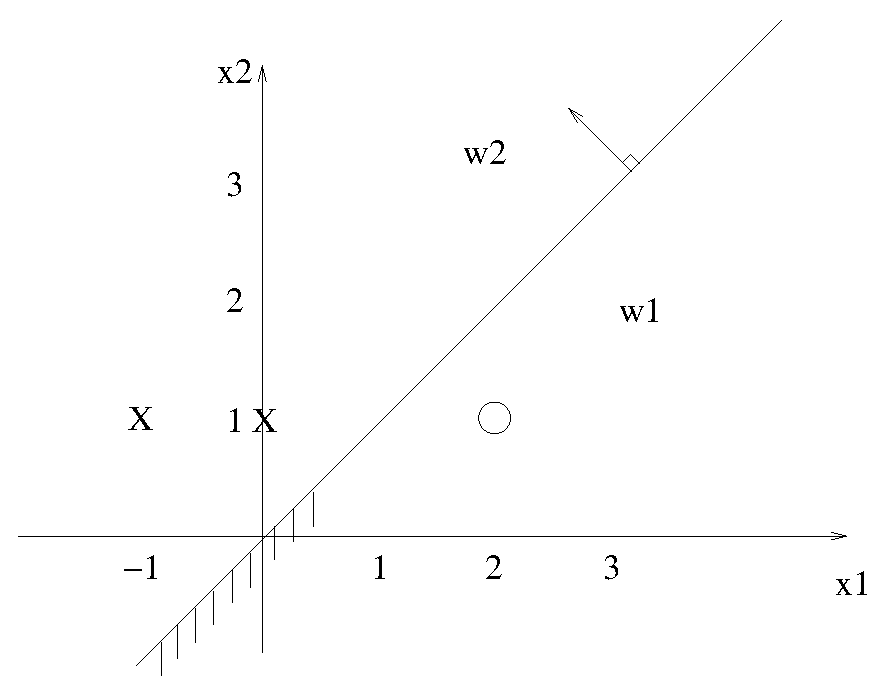
\includegraphics[scale=0.35]{e4_5}
      \end{center}

      Classifications are carried out as follows:
      \begin{equation*}
        \begin{cases}
          \vw^T\vx<0 \Rightarrow \vx \in \psi_1\\
          \vw^T\vx\geq 0 \Rightarrow \vx \in \psi_2\\
        \end{cases}
      \end{equation*}

    \item

      \begin{align}
        &\psi_1:\text{\;} \{ [1,1]^T, [2,2]^T \}, \notag \\
        &\psi_2: \text{\;} \{ [1,2]^T,[2,1]^T \} \notag
      \end{align}
      \begin{center}
        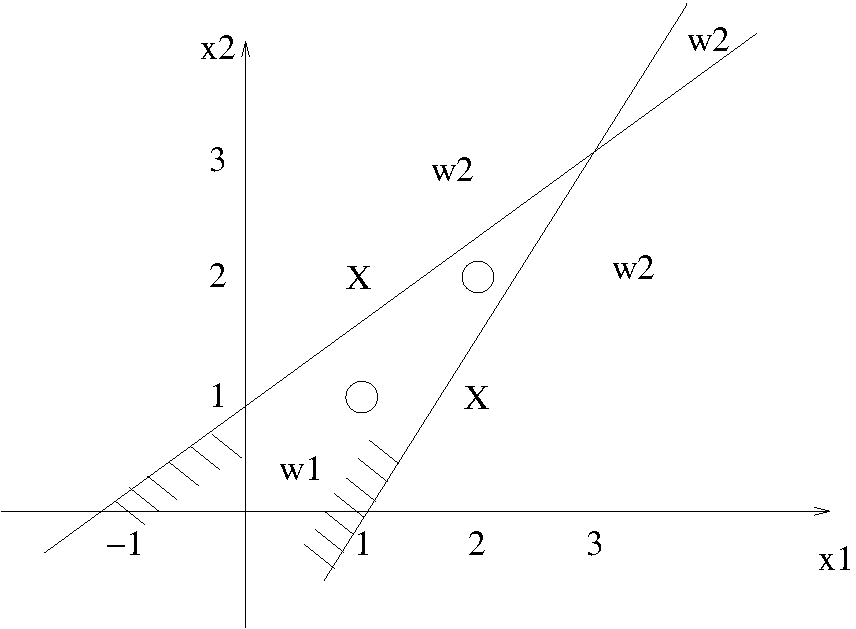
\includegraphics[scale=0.35]{e4_5b}
      \end{center}

      It is not possible to separate the classes with a single
      hyperplane. At least two hyperplanes are required to separated
      the classes correctly. In general, the sets are linearly
      separable if and only if the convex hulls of the sets do not
      overlap.  In this case, the convex hulls are the line segments
      connecting the two points in both sets.  These two line segments
      intersect at point $[1.5,1.5]^{\mathrm{T}}$, thus the sets are
      not linearly separable.

    \end{enumerate}

  \end{solution}


\item Consider the generative model
  \begin{equation*}
    x(n) = a x(n-1) + \epsilon(n)
  \end{equation*}
  which represents an autoregressive (AR) stochastic process of order
  one.  The only parameter of this process is $a$, which has in this
  simulation the value $a=0.99$.  The term $\epsilon(n)$ is zero mean
  white Gaussian noise having the variance $\sigma^2=0.02$,
  $\epsilon(n) \sim \mathrm{N}(0,\sigma^2)$, which drives the AR
  process.  Estimate the parameter $a$ of this AR process using the
  LMS algorithm.  Run the LMS algorithm with different learning rate
  parameter values $\mu =0.001, \, 0.01, \, 0.1, \, 1, \, 3$. Comment
  the results.

  \begin{solution}

    In order to make the analysis of the simulations more interesting,
    let us first examine theoretical bounds of convergence for $\mu$.
    Begin by computing the variance of $x(n)$ at ``equilibrium''
    (i.e., $\mathrm{E}[x(n)^2]=\mathrm{E}[x(n-1)^2]$):
    \begin{align*}
      C_x &= \mathrm{E}[x(n)^2]
      \\
      &= \mathrm{E}[a^2x(n-1)^2 + 2ax(n-1)\epsilon(n) + \epsilon(n)^2]
      \\
      &= a^2\mathrm{E}[x(n-1)^2] +
      2a\mathrm{E}[x(n-1)]\underbrace{\mathrm{E}[\epsilon(n)]}_{=0} +
      \mathrm{E}[\epsilon(n)^2]
      \\
      &= a^2 C_x + \sigma^2.
    \end{align*}
    Solve $C_x$:
    \begin{align*}
      C_x &= a^2C_x + \sigma^2
      \\
      (1-a^2)C_x &= \sigma^2
      \\
      C_x &= \frac{\sigma^2}{1-a^2} \approx 1.005.
    \end{align*}
    The process is stable when $1-a^2>0$, that is, $|a|<1$. Now
    $a=0.99$ so the process is stable.  By the theory of the LMS
    algorithm, in order for the LMS algorithm to converge, the
    learning parameter $\mu$ must satisfy
    \begin{equation*}
      0 < \mu < \frac{2}{C_x} \approx 1.99.
    \end{equation*}
    Below some comments:
    \begin{itemize}
    \item This theoretical bound assumes that the data points
      $x(n),x(n-1),\ldots,x(1)$ are independent.  In this case, they
      are \emph{not} independent, thus the theoretical bound does not
      hold.  In practice, the upper bound for $\mu$ is near $0.1$ as
      found by the simulations.
    \item The estimated parameter in a single run may not converge
      (even if the algorithm converges in the mean).  Because of the
      fixed learning parameter and the noise in the observations, the
      algorithm oscillates around the true solution.  Even if the
      oscillation is reduced by making $\mu$ smaller, the noise still
      causes some oscillation.  Thus, with small $\mu$ the mean
      squared-error converges close to the noise variance $0.02$.
    \item The squared error oscillates in a single simulation but one
      can approximate the \emph{mean} squared error by averaging over
      several runs, thus reducing the oscillation.  Note that it is
      the \emph{mean} squared error that converges, not the squared
      error of a single run.
    \item The mean squared error may converge to a large value.  If
      the learning parameter is large (but small enough for the
      algorithm to converge) the converged value may be very large
      (e.g., $10^5$).  Thus, the algorithm may perform extremely badly
      even if it converges.
    \item If the algorithm does not converge, the mean squared error
      increases without bounds as the iteration progresses and the
      parameter estimation ``explodes''.
    \item If the model was modified such that the data points are
      independent, the theoretical bound for $\mu$ seems to hold in
      practice (although the algorithm may perform badly).  This
      implementation is also available in the accompanied Matlab file.
    \end{itemize}
    
    \lstinputlisting[language=Matlab,
                     showstringspaces=false,
                     title=\lstname]{ex02_04.m}
  \end{solution}
  
% \item

%   \begin{enumerate}
%   \item
%     By substituting the optimal weights
%     \begin{equation}
%       \mathbf{w}_* = \mathbf{C}_x^{-1} \mathbf{p}
%       \label{eq:w_optimal}
%     \end{equation}
%     into the cost function
%     \begin{equation}
%       J(\mathbf{w}) = \frac{1}{2} \mathrm{E}\{d^2(n)\} -
%       \mathbf{p}^{\mathrm{T}}\mathbf{w} +
%       \frac{1}{2}\mathbf{w}^{\mathrm{T}} \mathbf{C}_x \mathbf{w}
%       \label{eq:J}
%     \end{equation}
%     prove that
%     \begin{equation}
%       J(\mathbf{w}_*) = \frac{1}{2} \mathrm{E}\{ d^2(n) \} - \frac{1}{2}
%       \mathbf{p}^T \mathbf{w}_*.
%       \label{eq:J2}
%     \end{equation}
    
%   \item Using \eqref{eq:J2}, prove that \eqref{eq:J} can be expressed as
%     \begin{equation*}
%       J(\mathbf{w}) = J(\mathbf{w}_*) + \frac{1}{2}( \mathbf{w} -
%       \mathbf{w}_*)^T \mathbf{C}_x (\mathbf{w} - \mathbf{w}_*)
%     \end{equation*}
%   \end{enumerate}

%   \begin{solution}

%     First, some background for the linear neuron:
%     \begin{itemize}
%     \item $\mathbf{x}(n)$ is the input vector at time $n$
%     \item $\mathbf{w}$ is the weight vector
%     \item $\mathbf{x}(n)^{\mathrm{T}} \mathbf{w}$ is the linear output
%       of the neuron at time $k$
%     \item $d(n)$ is the desired output at time $n$
%     \item $e(n)=d(n)-\mathbf{x}(n)^{\mathrm{T}} \mathbf{w}$ is the
%       error of the output at time $n$
%     \end{itemize}
%     Thus, the mean squared error (MSE) to be minimized can be given as
%     \begin{align*}
%       J(\mathbf{w}) 
%       &=\frac{1}{2}E[e^2(n)]
%       \\
%       &=\frac{1}{2}E[(d(n)-\mathbf{x}(n)^T\mathbf{w})^2]
%       \\
%       &=
%       \frac{1}{2} E[d(n)^2] - \mathbf{w}^T E[ d(n) \mathbf{x}(n)  ]  + 
%       \frac{1}{2} \mathbf{w}^T E[\mathbf{x}(n) \mathbf{x}(n)^T ] \mathbf{w} .
%     \end{align*}
%     % 
%     Now if we define 
%     \begin{equation*}
%       \mathbf{C}_x = E[\mathbf{x}(n) \mathbf{x}(n)^T ]
%     \end{equation*}
%     and
%     \begin{equation*}
%       \mathbf{p} = E[d(n) \mathbf{x}(n) ] ,
%     \end{equation*}
%     we get the MSE criterion as in equation \eqref{eq:J}
%     \begin{align*}
%       J(\mathbf{w}) = \frac{1}{2} E[d(n)^2] - \mathbf{p}^{\mathrm{T}} \mathbf{w}   + 
%       \frac{1}{2} \mathbf{w}^T \mathbf{C}_x \mathbf{w} .
%     \end{align*}
%     % 
%     Recall that the objective is to minimize the $J(\mathbf{w})$.  The
%     gradient of this is
%     \begin{align*}
%       \nabla_{\mathbf{w}} J =   \mathbf{C}_x \mathbf{w} - \mathbf{p} .
%     \end{align*}
%     % 
%     Now setting this to zero, we can solve for the minimizer of $J$ as
%     in equation \eqref{eq:w_optimal}:
%     \begin{equation*}
%       \mathbf{w}_* = \mathbf{C}_x^{-1} \mathbf{p} .
%     \end{equation*}
%     \begin{enumerate}
%     \item
%       Now, prove \eqref{eq:J2} by computing $J(\mathbf{w}_*)$:
%       \begin{align*}
%         J(\mathbf{w}_*) &= \frac{1}{2} E[d(n)^2] -
%         \mathbf{p}^{\mathrm{T}} \mathbf{w}_* + \frac{1}{2}
%         \mathbf{w}_*^T \mathbf{C}_x \mathbf{w}_*
%         \\
%         &= \frac{1}{2} E[d(n)^2] - \mathbf{p}^{\mathrm{T}}
%         \mathbf{w}_* + \frac{1}{2} \mathbf{p}^T
%         \cancel{\mathbf{C}^{-1}_x \mathbf{C}_x} \mathbf{w}_*
%         \\
%         &= \frac{1}{2} E[d(n)^2] - \frac{1}{2}\mathbf{p}^{\mathrm{T}}
%         \mathbf{w}_*
%       \end{align*}
%     \item
%       Let us prove by a straightforward calculation:
%       \begin{align*}
%         &\quad J(\mathbf{w}_*) + \frac{1}{2}( \mathbf{w} -
%         \mathbf{w}_*)^T \mathbf{C}_x (\mathbf{w} - \mathbf{w}_*)
%         \\
%         &= \frac{1}{2} \mathrm{E}\{ d^2(n) \} - \frac{1}{2}
%         \mathbf{p}^T \mathbf{w}_* + \frac{1}{2}\mathbf{w}^{\mathrm{T}}
%         \mathbf{C}_x \mathbf{w} -
%         \mathbf{w}_*^{\mathrm{T}}\mathbf{C}_x \mathbf{w} + \frac{1}{2}
%         \mathbf{w}^T_* \mathbf{C}_x\mathbf{w}_*
%         \\
%         &= \frac{1}{2} \mathrm{E}\{ d^2(n) \} - \cancel{\frac{1}{2}
%           \mathbf{p}^T \mathbf{w}_*} +
%         \frac{1}{2}\mathbf{w}^{\mathrm{T}} \mathbf{C}_x \mathbf{w} -
%         \mathbf{p}^{\mathrm{T}}\cancel{\mathbf{C}_x^{-1}\mathbf{C}_x}\mathbf{w}
%         + \cancel{\frac{1}{2} \mathbf{p}^T\mathbf{C}_x^{-1}
%           \mathbf{Cw}_*}
%         \\
%         &= \frac{1}{2} \mathrm{E}\{ d^2(n) \} +
%         \frac{1}{2}\mathbf{w}^{\mathrm{T}} \mathbf{C}_x \mathbf{w} -
%         \mathbf{p}^{\mathrm{T}}\mathbf{w}
%         \\
%         &= J(\mathbf{w})
%       \end{align*}

%       Alternatively, we may observe that $\nabla_{\mathbf{w}_*} J = 0$
%       and the Hessian of $J$ at $\mathbf{w}_*$ is $\mathbf{C}_x$.  The
%       higher order derivatives are zero, because $J$ is a second order
%       polynomial with respect to $\mathbf{w}$ and thus
%       \begin{equation*}
%         J(\mathbf{w}) = J( \mathbf{w}_* ) + \frac{1}{2} ( \mathbf{w} -
%         \mathbf{w}_* ) \mathbf{C}_x ( \mathbf{w} - \mathbf{w}_* ) . 
%       \end{equation*}
%     \end{enumerate}

%   \end{solution}
  
\end{enumerate}

\end{document}             % End of document.

%%% Local Variables: 
%%% mode: latex
%%% TeX-master: "ex02_solutions"
%%% End: 
